\chapter{Franck-Hertz-Versuch}


\section{Theoretischer Hintergrund}
Der Franck-Hertz-Versuch, erstmals 1914 von James Franck und Gustav Hertz durchgeführt, lieferte den ersten direkten experimentellen Nachweis für quantisierte Energieniveaus in Atomen. Er bestätigte die entstehende Quantentheorie, indem er zeigte, dass Elektronen nur diskrete Energiemengen an Atome übertragen können, um diese in angeregte Zustände zu versetzen.
\vspace{0.3cm}\\
In diesem Versuch werden Elektronen durch eine glühende Kathode über Thermoemission freigesetzt und durch eine Beschleunigungsspannung $U_B$ durch mit Quecksilberdampf gefülltes Gas beschleunigt. Auf ihrem Weg durch das Gas können die Elektronen mit Quecksilberatomen zusammenstoßen. Abhängig von ihrer Energie verlaufen diese Stöße entweder elastisch oder inelastisch.
\vspace{0.3cm}\\
Solange die Elektronen nicht genügend kinetische Energie haben, um ein Atom anzuregen, finden nur elastische Stöße statt, bei denen die Elektronen nahezu keine Energie verlieren. Überschreiten sie jedoch die Anregungsenergie des Atoms, kommt es zu inelastischen Stößen, bei denen ein Elektron eine definierte Energiemenge an das Atom abgibt und dieses in einen angeregten Zustand überführt. Das Atom kehrt anschließend durch Emission eines Photons in den Grundzustand zurück, während das Elektron mit verminderter kinetischer Energie weiterfliegt.
\vspace{0.3cm}\\
Die niedrigste Anregungsenergie des Quecksilberatoms liegt bei etwa
\begin{equation}
\Delta E \approx \SI{4.9}{\electronvolt} 
\end{equation}
und entspricht dem Übergang vom Grundzustand $6^1S_0$ in den angeregten Zustand $6^3P_1$ \cite{hg_EE}.
\vspace{0.3cm}\\
Bevor die Elektronen die Anode erreichen, müssen sie eine kleine Gegenspannung $U_G$ überwinden. Elektronen, die durch inelastische Stöße zu viel Energie verlieren, können diese Barriere nicht überwinden und tragen daher nicht zum gemessenen Anodenstrom $I_A$ bei.
\vspace{0.3cm}\\
Wenn die Beschleunigungsspannung $U_B$ schrittweise erhöht wird, steigt der Anodenstrom zunächst an, da mehr Elektronen die Anode erreichen. Sobald $e U_B \geq \SI{4.9}{\electronvolt}$ ist, beginnen inelastische Stöße $\rightarrow$ einige Elektronen verlieren Energie $\rightarrow$ weniger Elektronen überwinden $U_G$ $\rightarrow$ $I_A$ sinkt. Mit weiter steigender Spannung gewinnen die Elektronen erneut genug Energie $\rightarrow$ $I_A$ steigt wieder, bis eine zweite Anregung möglich wird $\rightarrow$ zweites Minimum. So entsteht eine periodische Folge von Maxima und Minima im Strom-Spannungs-Diagramm.
\vspace{0.3cm}\\
Der Abstand zwischen zwei benachbarten Maxima oder Minima entspricht der Anregungsenergie:
\begin{equation}
\Delta E = e \cdot \Delta U
\end{equation}
\vspace{0.3cm}\\
Die kinetische Energie der Elektronen ergibt sich aus:
\begin{equation}
E_{\text{kin}} = e \cdot U_B
\end{equation}
\vspace{0.3cm}\\
Die Temperatur beeinflusst über den Dampfdruck die mittlere freie Weglänge der Elektronen. Ein höherer Dampfdruck (bei höherer Temperatur) führt zu häufigeren Stößen, wodurch die Maxima in der Stromkurve unschärfer werden. Ist die Temperatur zu niedrig, finden kaum Stöße statt und es erscheint keine Struktur im Stromverlauf.
\vspace{0.3cm}\\
Die mittlere freie Weglänge $\lambda$ lässt sich näherungsweise berechnen durch:
\begin{equation}
\lambda = \frac{k_B T}{\sqrt{2} \pi d^2 p}
\end{equation}
mit $k_B$ als Boltzmann-Konstante, $T$ der Temperatur, $d$ dem Atomdurchmesser und $p$ dem Dampfdruck.
\vspace{0.3cm}\\
Die Gegenspannung $U_G$ wirkt als Filter für langsame Elektronen. Eine Erhöhung von $U_G$ reduziert den gemessenen Strom, verändert jedoch nicht die Lage der Maxima.
\vspace{0.3cm}\\
% ----------------------------------------------------------------------------------
% ----------------------------------------------------------------------------------
% ----------------------------------------------------------------------------------
% ----------------------------------------------------------------------------------
% ----------------------------------------------------------------------------------
% ----------------------------------------------------------------------------------
\section{Aufbau}

\begin{figure}[H]
    \centering
    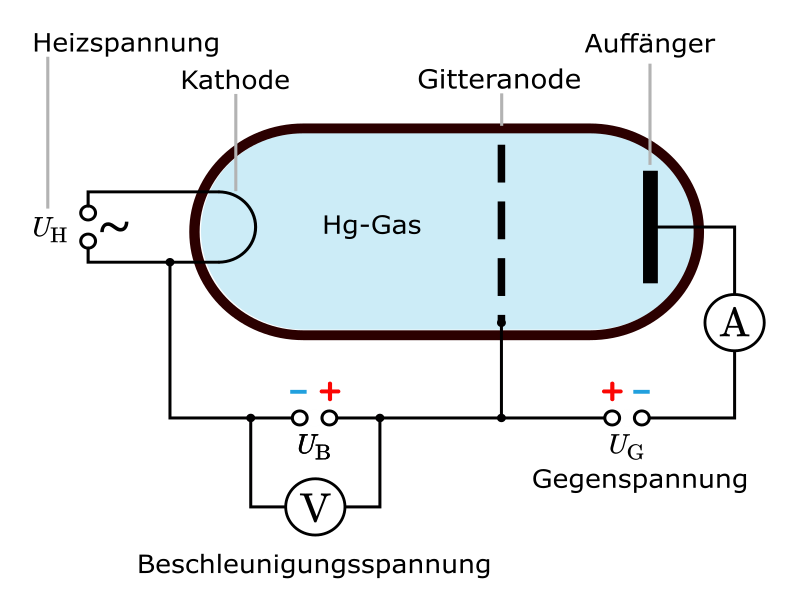
\includegraphics[width=0.5\textwidth]{FranckHertz.png}
    \caption{Schematischer Aufbau vom Frank-Hertz-Versuch \cite{FranckHertzHg}} 
    \label{fig:FrankHertzSchaltung}    
\end{figure}

Der experimentelle Aufbau (schematisch in \cref{fig:FrankHertzSchaltung}) besteht aus einer mit Quecksilberdampf (Hg-Gas) gefüllten Franck-Hertz-Röhre, die sich in einem temperaturgeregelten Ofen befindet. Elektronen werden durch Glühemission aus einer beheizten Kathode freigesetzt und mit einer einstellbaren Beschleunigungsspannung $ U_B $ in Richtung eines Gitters beschleunigt. Nach dem Passieren des Gitters stoßen die Elektronen auf eine kleine Gegenspannung $ U_G $, bevor sie die Anode erreichen.
\vspace{0.3cm}\\
Die Gegenspannung $ U_G $ stellt sicher, dass nur Elektronen mit ausreichend kinetischer Energie - also solche, die keine oder nur elastische Stöße erfahren haben - die Anode erreichen können. Der resultierende Anodenstrom $ I_A $ wird mit einem empfindlichen Amperemeter gemessen. Die Beschleunigungsspannung $ U_B $ wird mit einem Voltmeter überwacht.
\vspace{0.3cm}\\
Der Ofen ermöglicht die präzise Temperaturregelung des Quecksilberdampfes, was entscheidend ist, da die Dampfdruckabhängigkeit die mittlere freie Weglänge der Elektronen beeinflusst. Eine konstante Temperatur ist notwendig, um reproduzierbare und deutlich sichtbare Maxima in der Franck-Hertz-Kurve zu erhalten.
\vspace{0.3cm}\\
Die gesamte Apparatur wird über eine externe Steuereinheit betrieben, die das automatische Hochfahren der Beschleunigungsspannung sowie eine synchrone Datenaufnahme über die Messsoftware erlaubt.
\vspace{0.3cm}\\
% ----------------------------------------------------------------------------------
% ----------------------------------------------------------------------------------
% ----------------------------------------------------------------------------------
% ----------------------------------------------------------------------------------
% ----------------------------------------------------------------------------------
% ----------------------------------------------------------------------------------

\section{Durchführung}

Zu Beginn des Experiments wird der Franck-Hertz-Ofen auf etwa \SI{165}{\celsius} aufgeheizt und thermisch stabilisiert, um während der Messung einen konstanten Quecksilberdampfdruck sicherzustellen. Zwei Messmodule (Cassy-Einheiten) zur Erfassung von Spannung und Strom werden mit den Anschlüssen der Ofeneinheit verbunden. Diese Module sind wiederum mit einem Computer verbunden, auf dem die Cassy Lab Software ausgeführt wird. In der Software wird die vorkonfigurierte Datei \textit{"Franck Hertz"} geladen, welche die Datenaufnahme und die Gerätesteuerung übernimmt.
\vspace{0.3cm}\\
Sobald das System im Gleichgewichtszustand ist, wird die Messung durch Drücken der Schaltfläche \textit{"Messung starten"} (F9) in der Softwareoberfläche gestartet. Dieser Schritt aktiviert die Datenerfassung. Anschließend wird der \textit{''Start/Stop''}-Knopf an der Hardware-Steuereinheit des Ofens gedrückt. Dadurch wird die automatische Rampe der Beschleunigungsspannung $U_B$ von \SI{0}{\volt} bis zu einem vorher festgelegten Maximalwert ausgelöst. Während dieses Spannungshubs werden Elektronen aus der beheizten Kathode emittiert, durch den Quecksilberdampf beschleunigt und erreichen entweder die Anode oder werden - abhängig von ihrer kinetischen Energie nach einem Stoß und der angelegten Gegenspannung $U_G$ - zurückgehalten. Der Anodenstrom $I_A$ wird kontinuierlich als Funktion von $U_B$ gemessen und aufgezeichnet und liefert so eine direkte Darstellung der Energieverluste der Elektronen durch Stoßprozesse im Dampf.
\vspace{0.3cm}\\
Es werden zwei getrennte Messreihen durchgeführt, um den Einfluss experimenteller Parameter zu untersuchen. Zunächst werden $I_A(U_B)$-Kurven für vier verschiedene Werte der Gegenspannung $U_G$ (im Bereich von \SIrange{2}{4}{\volt}) bei konstanter Ofentemperatur aufgenommen. Danach wird das Experiment bei vier verschiedenen Temperaturen (zwischen \SI{165}{\celsius} und \SI{180}{\celsius}) mit einer festen Gegenspannung wiederholt. Jede Messung sollte eine Anodenstromkurve liefern, die mindestens vier ausgeprägte Maxima zeigt, welche auf aufeinanderfolgende inelastische Anregungen von Quecksilberatomen durch die einfallenden Elektronen zurückzuführen sind.
\vspace{0.3cm}\\
Während der Datenerfassung ist darauf zu achten, Anzeichen für einen elektrischen Durchbruch in der Röhre zu erkennen. Ein plötzlicher Anstieg des Anodenstroms oder ein bläuliches Leuchten in der Röhre weist auf Ionisation oder Gasdurchschlag hin. Tritt ein solcher Zustand auf, muss die Messung sofort durch Drücken des \textit{Start/Stop}-Knopfs beendet werden. Der Maximalwert der Beschleunigungsspannung $U_B$ ist anschließend zu reduzieren (auf unter $\approxeq\SI{45}{\volt}$), um einen erneuten Durchbruch zu vermeiden. Die Messung kann dann mit angepassten Parametern wiederholt werden.
\vspace{0.3cm}\\
Alle Datensätze sollten unmittelbar nach der Aufnahme gespeichert werden, wobei die Dateinamen die jeweiligen experimentellen Bedingungen ($U_G$ und Temperatur) eindeutig widerspiegeln. Diese Datensätze bilden die Grundlage für die weitere quantitative Auswertung der Anregungsenergie und des Einflusses experimenteller Parameter auf das charakteristische Strom-Spannungs-Verhalten der mit Quecksilber gefüllten Franck-Hertz-Röhre.
% ----------------------------------------------------------------------------------
% ----------------------------------------------------------------------------------
% ----------------------------------------------------------------------------------
% ----------------------------------------------------------------------------------
% ----------------------------------------------------------------------------------
% ----------------------------------------------------------------------------------
\section{Auswertung}


\subsection*{Bestimmung der Anregungsenergie $\Delta E$ von Quecksilber}

Zur Bestimmung der Anregungsenergie des Quecksilberatoms wurde der Anodenstrom $I_A$ als Funktion der Beschleunigungsspannung $U_B$ für verschiedene Einstellungen aufgenommen. Die erhaltenen Franck-Hertz-Kurven zeigen eine Reihe periodischer Maxima, die jeweils dem Zustand entsprechen, in dem die Elektronen genügend kinetische Energie erworben haben, um ein Quecksilberatom durch inelastische Stöße anzuregen. Durch Bestimmen der Positionen mindestens fünf aufeinanderfolgender Maxima in den gemessenen $I_A(U_B)$-Kurven lässt sich der Spannungsabstand $\Delta U$ zwischen den Peaks ermitteln. Dieser Abstand spiegelt direkt die zur Anregung des Atoms vom Grundzustand in den ersten angeregten Zustand benötigte Energie wider. Die Anregungsenergie ist $\Delta E$. 
\vspace{0.3cm}\\
In diesem Experiment wurde ein mittlerer Spannungsabstand gefunden, woraus sich eine Anregungsenergie ergibt (werte sind in \cref{tab:franckU2} und \cref{tab:franckT}). Dieser Wert liegt im guten Einklang mit der bekannten Anregungsenergie des Übergangs $6^1S_0 \to 6^3P_1$ im Quecksilberatom, welcher bei etwa $4{,}9\,\mathrm{eV}$ liegt (\cref{fig:Hg_energyLevels}).
\vspace{0.3cm}
\begin{figure}[H]
    \centering
    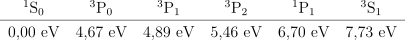
\includegraphics[width=0.5\textwidth]{figs/EnergieniveausvonQuecksilber.png}
    \caption{Energieniveaus von Quecksilber (\cite{praktikum4}) }
    \label{fig:Hg_energyLevels}
\end{figure}

Die Spannungsunsicherheiten wurden auf $\pm 2\%$ des Messbereichs und zusätzlich auf $\pm 0.5\%$ des maximal gemessenen Werts geschätzt, in Übereinstimmung mit den Spezifikationen des Cassy-Moduls. Zur Bestimmung von $\Delta E$ wurden die fünf höchsten Maxima jeder Anodenspannungskurve mit einer einzelnen Gaußfunktion angepasst:

\begin{equation}
  U_A = O + A \exp\!\biggl[-\frac{(U_B - \mu)^2}{2\,\sigma^2}\biggr],
\end{equation}

\noindent wobei $O$ der Offset, $A$ die Amplitude, $\mu$ die Peakposition und $\sigma$ die Standardabweichung des Peaks ist. Die Anregungsenergie ergibt sich dann aus
\vspace{0.3cm}
\begin{equation}
  \Delta E = e \,\Delta U_B,
\end{equation}
\vspace{0.3cm}
\noindent wobei $\Delta U_B$ die Differenz der mittels $\mu$ bestimmten Peakpositionen ist. \cref{tab:franckU2} und \cref{tab:franckT} fasst die mittleren Werte von $\Delta E$ sowie die entsprechenden Breiten $\sigma$ zusammen.
\vspace{0.3cm}\\
Die anderen Übergänge treten seltener auf, was durch den Gesamtwirkungsquerschnitt von Quecksilber für die Elektronenstoßanregung erklärt werden kann (\cref{fig:Querschnitt}). 
Da die Elektronen kontinuierlich Energie verlieren, ist der Gesamtwirkungsquerschnitt im Energiebereich der Übergänge 1, 2 und 3 am höchsten. Daher liegt unser gemittelter Wert genau in der Mitte dieses Bereichs. Übergang 4 wird erst bei höheren Energien relevant.

\begin{figure}[H]
  \centering
  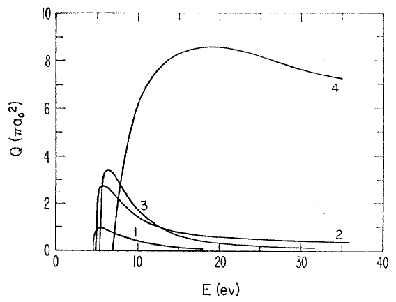
\includegraphics[width=0.5\textwidth]{figs/TotalerWirkungsquerschnitt.png}
  \caption{Totaler Wirkungsquerschnitt von Hg für Elektronenstoßanregung(\cite{praktikum4}).}
  \label{fig:Querschnitt}
\end{figure}

\subsection*{Abhängigkeit der Gegenspannung}

In \cref{fig:UGall} sind alle Anodenstromkurven für unterschiedliche Gegenspannungen zusammen dargestellt. Man erkennt deutlich, dass das Stromniveau mit steigender Gegenspannung abfällt. Das ist nachvollziehbar, da eine höhere Gegenspannung verhindert, dass Elektronen die Anodenplatte erreichen und so Strom erzeugen. Außerdem verschiebt sich jedes Maximum mit zunehmender Gegenspannung leicht zu höheren Beschleunigungsspannungen (also nach rechts).

\subsection*{Abhängigkeit der Temperatur}

In \cref{fig:Tall} zeigt sich, dass die Amplitude der Anodenstrommaxima mit steigender Temperatur abnimmt. Dieses Verhalten lässt sich folgendermaßen erklären: Bei höheren Temperaturen steigt der Quecksilberdampfdruck gemäß

\begin{equation}
\log p = 10.55 - \frac{3333}{T} - 0.85\,\log T
\end{equation}

\noindent wobei $p$ in Torr und $T$ in Kelvin angegeben ist \cite{praktikum4}. Mit steigendem Dampfdruck wird die mittlere freie Weglänge der Elektronen kürzer, sodass sie im Mittel weniger kinetische Energie gewinnen. Dies führt zu kleineren und breiteren Maxima in der Anodenstromkurve, genau wie beobachtet.
\vspace{0.3cm}\\
Aus den Werten in Tabelle 4 ergibt sich, dass der totale Wirkungsquerschnitt für den Übergang $^1S_0 \to {}^3P_0$ bei kleineren Elektronenenergien noch deutlicher ausgeprägt ist. Deshalb liegt unsere gemessene Anregungsenergie um etwa $4,9$V.
\vspace{0.3cm}\\
Setzt man die Dampfdruckgleichung bei $T = 165\,^\circ\mathrm{C}$ ein, erhält man einen Quecksilberdampfdruck von etwa $0,11$Torr; eine Erhöhung der Temperatur um $20$K erhöht den Druck auf ca. $0,15$Torr. Sowohl die Gleichung als auch unsere Messdaten zeigen, dass der Dampfdruck beträchtlich schwanken kann. Solche Druckänderungen beeinflussen, wie weit sich die Elektronen im Mittel zwischen zwei Stößen bewegen und damit, welche Anregungsprozesse stattfinden können. Die Untersuchung weiterer Übergänge liegt jedoch nicht im Fokus dieses Experiments - wir konzentrieren uns auf die Beobachtung eines einzelnen Energieübergangs.


Im Quecksilber-Franck-Hertz-Versuch ergibt sich das enge Temperaturintervall daraus, dass der Quecksilber­dampfdruck $p(T)$ mit der Temperatur $T$ exponentiell ansteigt und dadurch die mittlere freie Weglänge $\lambda$ der Elektronen drastisch abnimmt. Bereits wenige Kelvin Toleranz über oder unter der Optimaltemperatur führen zu $\lambda\gg L$ (kaum inelastische Stöße) bzw. $\lambda\ll L$ (Übermaß an elastischen und Mehrfachstößen, Raumladung und Strahlungsrückhaltung), sodass die scharf ausgeprägten Strommaxima entweder ganz ausbleiben oder verschmiert werden. Nur in einem engen Temperaturbereich sind die Stoßbedingungen so gewählt, dass die Elektronen gerade genügend kinetische Energie zwischen den Kollisionen sammeln und abgeben, um klar erkennbare Franck-Hertz-Maxima zu erzeugen.
